\documentclass{beamer}

\mode<presentation>
{
  \usetheme{Antibes}
  \setbeamercovered{transparent}
}

\usepackage[english]{babel}
\usepackage[latin1]{inputenc}
\usepackage{times}
\usepackage[T1]{fontenc} 
% Or whatever. Note that the encoding and the font should match. If T1
% does not look nice, try deleting the line with the fontenc.
\usepackage{amsmath}

\newcommand{\linespace}{\vskip 0.25cm}

\definecolor{MyForestGreen}{rgb}{0,0.7,0} 
\newcommand{\mynotes}[1]{}

% The text in square brackets is the short version of your title and will be used in the
% header/footer depending on your theme.
\title[Interoperability]{Interoperability in Programming Languages}

% Sub-titles are optional - uncomment and edit the next line if you want one.
% \subtitle{Why does sub-tree crossover work?} 

% The text in square brackets is the short version of your name(s) and will be used in the
% header/footer depending on your theme.
\author[Malone]{Todd Malone}

% The text in square brackets is the short version of your institution and will be used in the
% header/footer depending on your theme.
\institute[U of Minn, Morris]
{
  Division of Science and Mathematics \\
  University of Minnesota, Morris \\
  Morris, Minnesota, USA
}

% The text in square brackets is the short version of the date if you need that.
\date[April '14, Senior Sem] % (optional)
{28 April 2014 \\ Senior Seminar}

% Delete this, if you do not want the table of contents to pop up at
% the beginning of each subsection:
\AtBeginSection[]
{
  \begin{frame}<beamer>
    \frametitle{Outline}
    \tableofcontents[currentsection, hideothersubsections]
  \end{frame}
}

\begin{document}

\begin{frame}
  \titlepage
\end{frame}

% For a 20-25 minute senior seminar talk you probably want something like:
% - Two or three major sections (other than the summary).
% - At *most* three subsections per section.
% - Talk about 30s to 2min per frame. So there should probably be between
%   15 and 30 frames, all told.
% Slide notes will be comment under each frame end, or under each column where appropriate.

\section*{Interoperability}

\subsection*{Introduction to Interop}

\begin{frame}
  \frametitle{What is Interop?}
  
  \begin{columns}
  \begin{column}{0.6\textwidth}
  \begin{itemize}
  	\item Interoperability or Interop
  	\item The ability for a system to use parts from another system
	\item In programming languages: The ability of a language to call on code from another language
  \end{itemize}
  \end{column}
%mainly, a program running in one language has the ability to call on aspects of another program, written in a different language  
  
  \begin{column}{0.4\textwidth}
   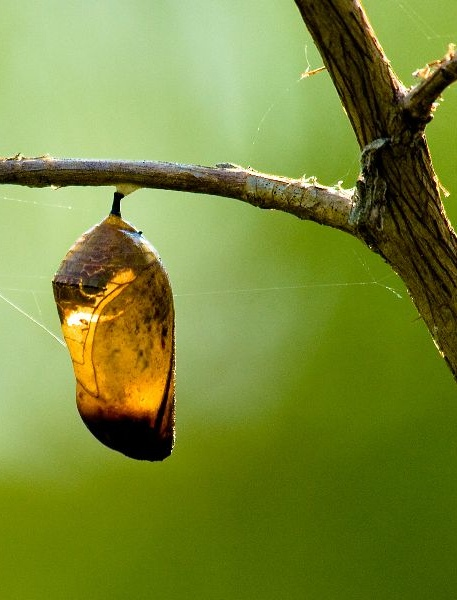
\includegraphics[width=0.90\textwidth]{graphics/Empty_cocoon_crop_by_Bluedrakon_from_Flickr.jpg}
       \\
    \only{\tiny{Bluedrakon \\ \url{http://tr.im/pWUi} }}
  \end{column}
  \end{columns}
\end{frame}

\begin{frame}
  \frametitle{Why is Interop Important?}
%These generally fall under to main categories: Dev time, or effort; and the purpose of different languages.
  
  \begin{columns}[t]
  \begin{column}{0.5\textwidth}
  Developer time and effort
  \begin{itemize}
	\item Existing and working code is easier to use as-is.
  	\item Third-party systems: source code is unavailable
	\item Legacy systems: extensive or little-understood code base.
  \end{itemize}
  \end{column}
  %existing (and working) code that does the thing you need it to do, it's easier to use as it is than it is to rewrite it.
  %sometimes, rewriting is an option, but there's just too much code and domain knowledge involved. (example: that a polygon doesn't cross itself) (if there's a lot, it would take a long time, too)
  %other time, you 

  \begin{column}{0.5\textwidth}
  Language Purpose:
  \begin{itemize}
  	\item Low-level memory access (C)
  	\item Parallel or distributed systems (Erlang, Clojure)
  	\item Statistics (R)
  \end{itemize}
  \end{column}
  \end{columns}
%
%each of these languages has some drawbacks, which not hugely importnant
%however, if the programmer isn't comfortable enough with the language to deal with its escentricities,
%then they'd be better served by utilizing it for the specific thing they need from it, in as small a chunk as they can get.

  
\end{frame}

\subsection*{Outline}

\begin{frame}
  \frametitle{Outline}
  \tableofcontents[hideallsubsections]
\end{frame}
%I'll be talking about two particular tools used for enabling interoperability,
%as well as two particular concepts central to interop in programming languages

\section[Interop Tools]{Tools used in achieving interoperability}

\subsection{Virtual Machines}

\begin{frame}
  \frametitle{Virtual Machines}
  
  %add graphic: CLR VM
  \begin{columns}
  \begin{column}{0.6\textwidth}
  \begin{itemize}
	\item Virtual Machines (VMs) are a runtime environment for a program
	\item High-level languages compile to an intermediate language
	\item Intermediate language: Java bytecode or Common Intermediate Language
  \end{itemize}
  \end{column}
  
  \begin{column}{0.5\textwidth}
  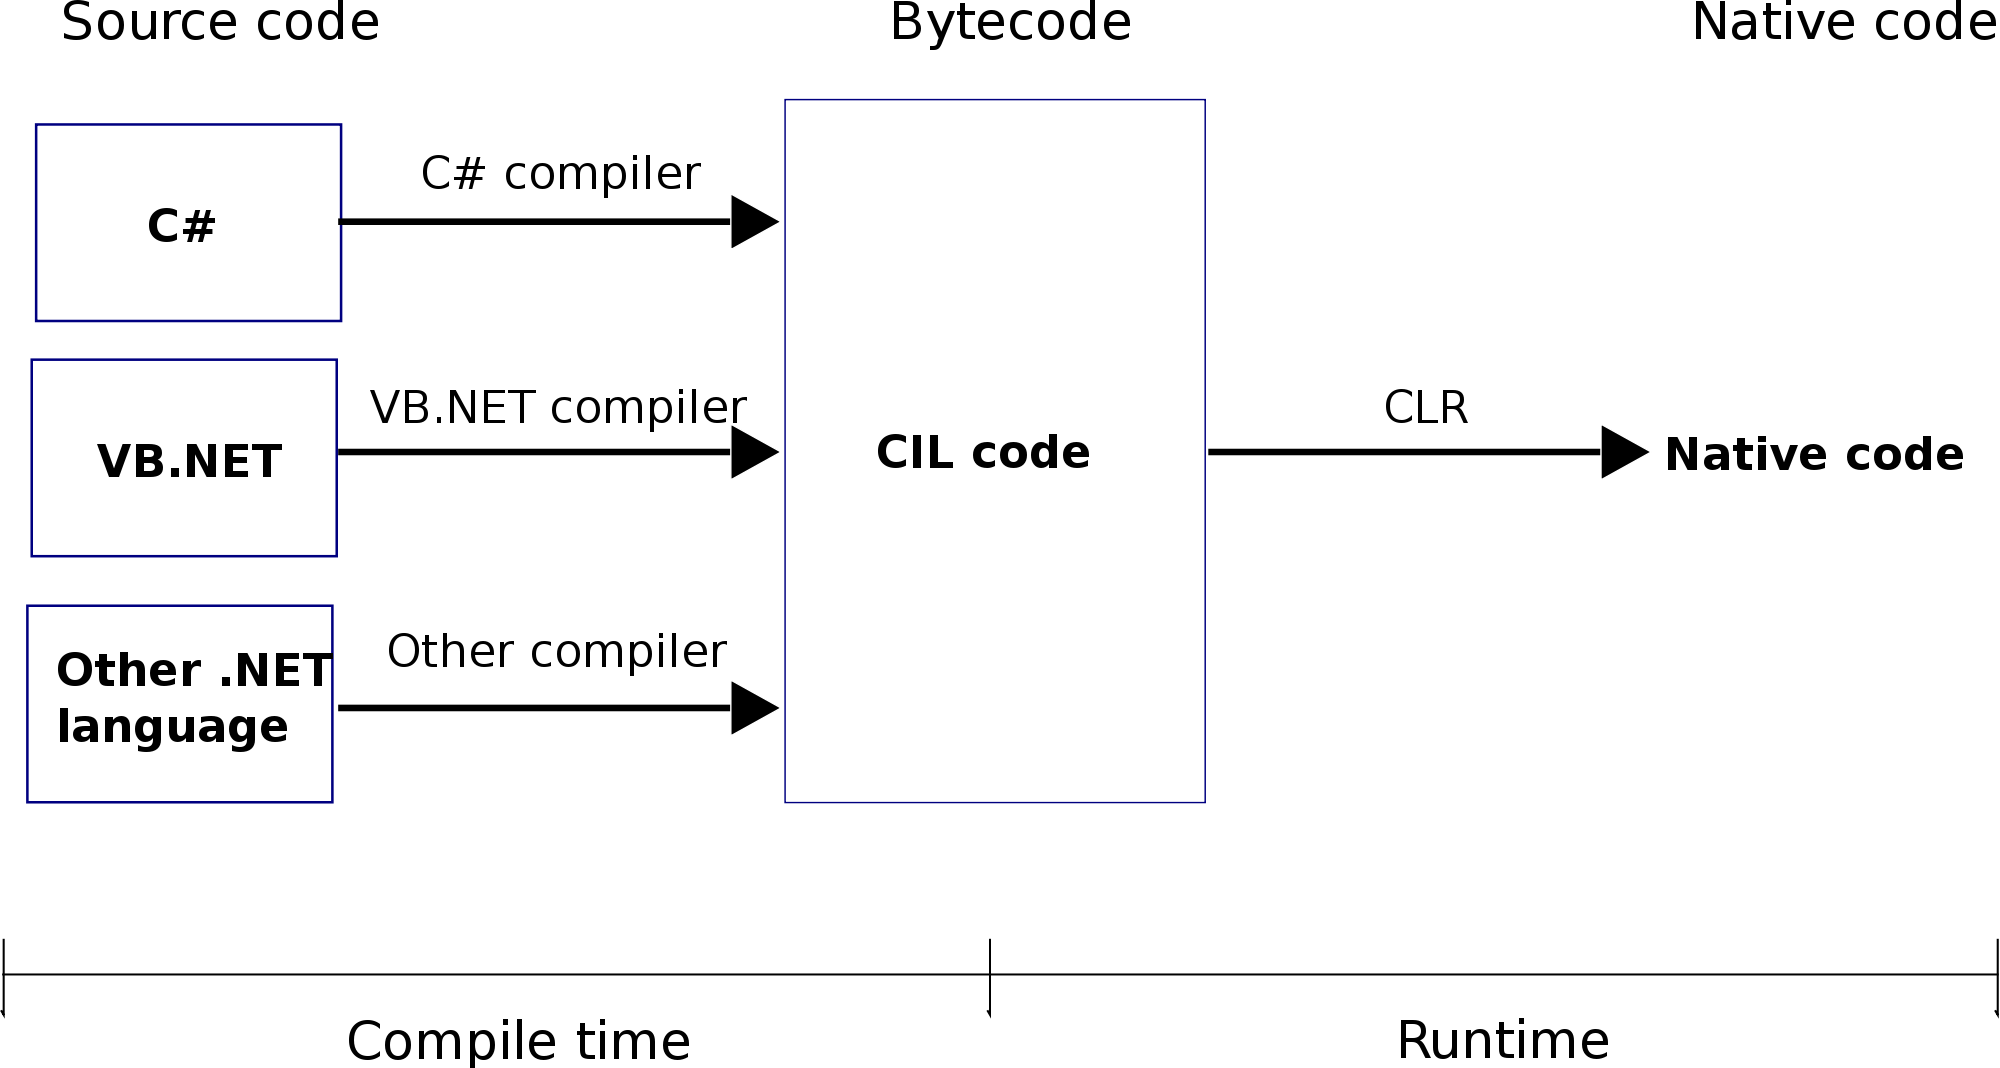
\includegraphics[width=1\textwidth]{graphics/CLR.png}
    \\
    \only{\tiny{Wikipedia \\ \url{https://en.wikipedia.org/wiki/Common_Language_Runtime}}}
  \end{column}
  \end{columns}
\end{frame}
%Briefly, VMs emulate an operating system, or computer hardware. We'll be talking about a specific kind of VM, the process VM, that acts as a runtime environment for a program.

\begin{frame}
  \frametitle{High-level vs Bytecode}
  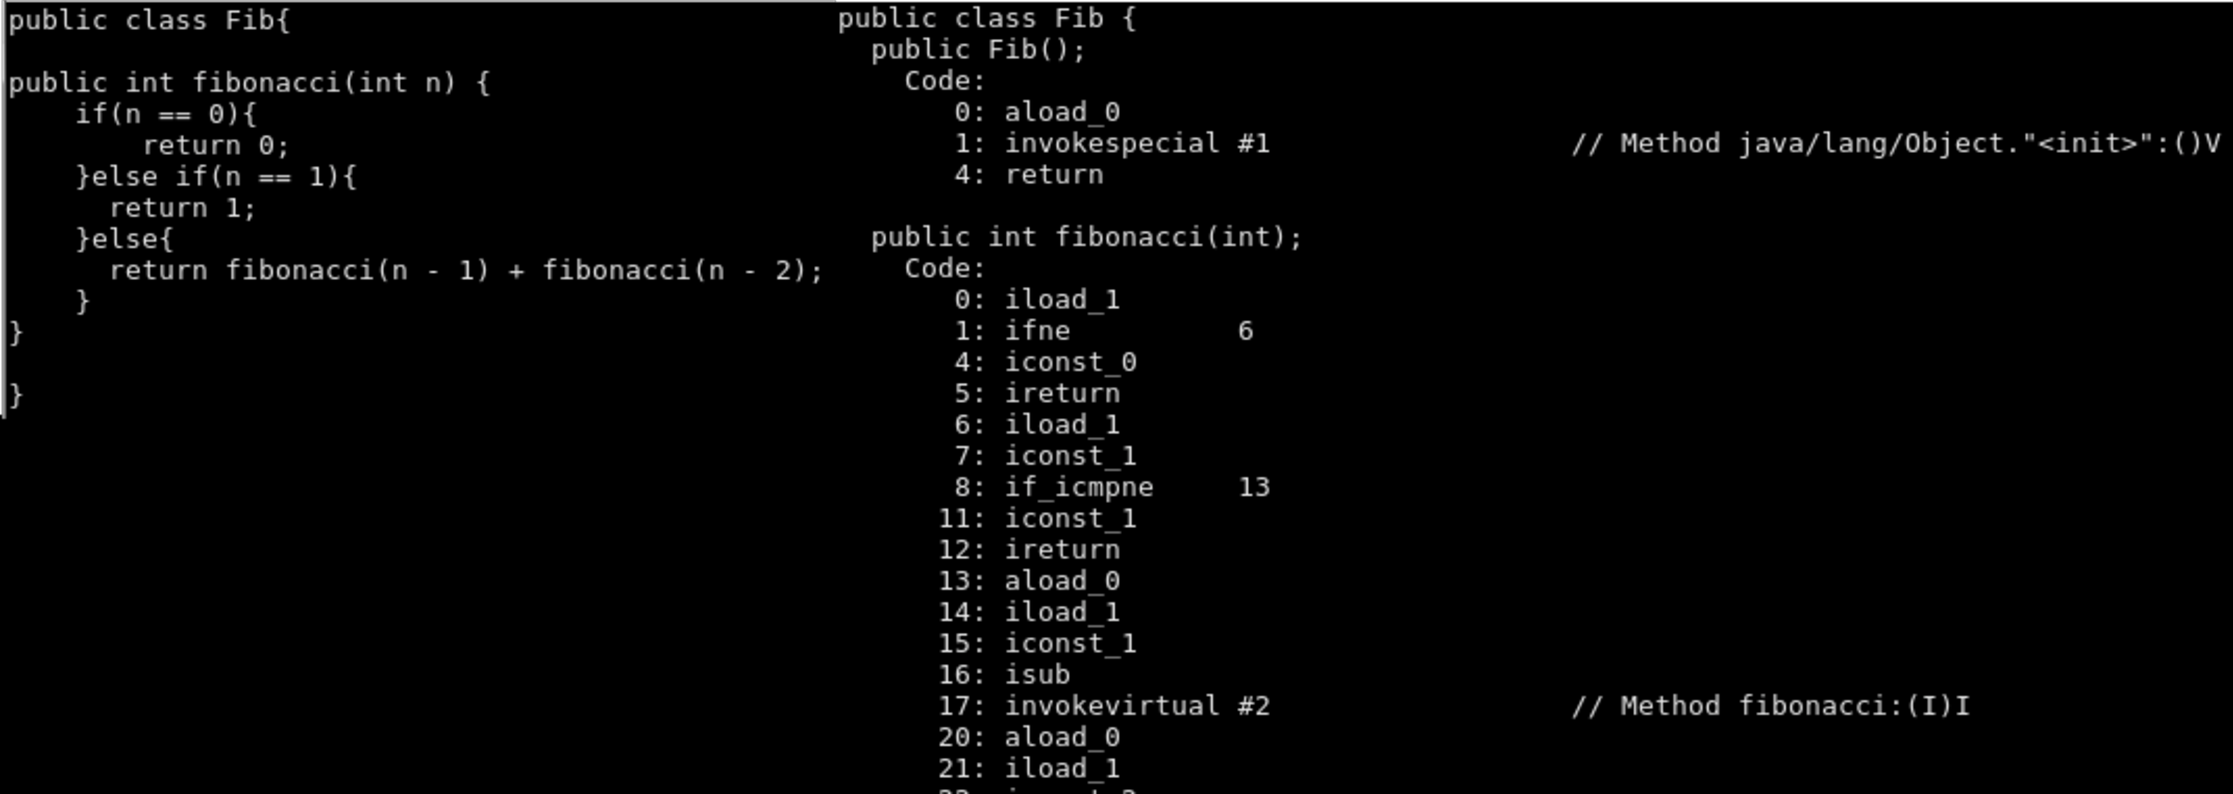
\includegraphics[width=1\textwidth]{graphics/FibCompair.pdf}
\end{frame}

\subsection{Markup Languages}

\begin{frame}[fragile]
  \frametitle{Markup Languages}
  
  \begin{columns}
  \begin{column}{0.5\textwidth}
  \begin{itemize}
	\item Markup languages are a way of modeling data.
	\item XML and JSON can model data like objects.
	\item Markup languages are independent of programming languages.
  \end{itemize}
  \end{column}

  \begin{column}{0.5\textwidth}
%this should be examples of Cliff in XML and JSON. If they don't fit, make them a new slide?
  \end{column}
  \end{columns}
  
\end{frame}
%MLs are mostly a way of annotating data in a way that another program can interpret that meaningfully, handle it accordingly.
%one of the emergent properties of this, in the form of XML, is the ability to model data in a way that it can be converted to a data structure in the reciving program.
%Several other languages have emerged to model data specifically in this way, like JSON. JSON is JavaScript's Object Notation, implying correctly that it models data like an object.


\section[Difficulties]{Common difficulties in interop}
%Everything in this section is closely related: it's all about the data.
%The three main problems encountered in 


\subsection{Type systems}
\begin{frame}
  \frametitle{Types (and untypes)}
  
  \begin{columns}
  \begin{column}{0.6\textwidth}
  \begin{itemize}
  	\item Languages represent data in different ways %numbers: Java says "int!", JavaScript says "Number!". Ruby says "Whatever! I'll figure it out."
	\item Languages act on data in different ways %This is most obvious in numbers, but Java and C# handle printing of NULL objects very differently
	\item 
	\item 
	\item 
  \end{itemize}
  \end{column}
  
  \begin{column}{0.5\textwidth}
  
  \end{column}
  \end{columns}
\end{frame}
%Numbers are really the easiest example, because there are so many ways of representing them. 

\subsection{Data structures}
\begin{frame}
  \frametitle{Types (and untypes)}
  
  \begin{columns}
  \begin{column}{0.6\textwidth}
  \begin{itemize}
  	\item 
	\item 
	\item 
	\item 
	\item 
  \end{itemize}
  \end{column}
  
  \begin{column}{0.5\textwidth}
  
  \end{column}
  \end{columns}
\end{frame}

\subsection{Data processing}
\begin{frame}
  \frametitle{Handling data}
  
  \begin{columns}
  \begin{column}{0.5\textwidth}
  \begin{itemize}
  \item Languages 
  \end{itemize}
  \end{column}
  \end{columns}
\end{frame}

\section[Handling interop]{Concepts in overcoming difficulties}

\subsection{Metadata}

\begin{frame}
  \frametitle{Metadata and type conversion}

	Metadata: Data about data
	
	{\tt (def mylist [1, 2, 3, 4])}
	
	{\tt (with-meta mylist \{:length 4, :type Integer\})}
	\linespace
	In Clojure:
	\begin{itemize}
	\item lists are untyped; can contain entries of different types.
	\item metadata, added as above, is all user-controlled.
	\end{itemize}
\end{frame}
%Metadata: data about data. Specifically, it's information beyond what the data itself can convey.
%Say we had x = 5. all x knows is that it's a five. "Integer" is a storage mechanism, or representation in the language.
%"Integer" is also context specific. Java knows about x's integer-ness, but JavaScript, or JSON, does not. 


\begin{frame}
    \frametitle{Why Metadata?}
  \begin{columns}
  \begin{column}{0.6\textwidth}

    \begin{itemize}   
    \item Decontextualized data can carry context with it
    \item Data transfer between languages with different type strictness.
    \end{itemize}
  \end{column}
   %add example here...
  \begin{column}{0.6\textwidth}
  
  \end{column}
  
  \end{columns}
\end{frame}

\subsection{Standards}

\begin{frame}
  \frametitle{The importance of Standards}
  
  \begin{columns}
  \begin{column}{0.6\textwidth}
  \begin{itemize}
  	\item 
	\item 
	\item 
	\item 
	\item 
  \end{itemize}
  \end{column}
  \end{columns}
\end{frame}

\section[Conclusions]{Conclusions}

\begin{frame}
  \frametitle{Conclusions}
  
  \begin{columns}
  \begin{column}{0.6\textwidth}
  \begin{itemize}
  	\item 
	\item 
	\item 
	\item 
	\item 
  \end{itemize}
  \end{column}
  \end{columns}
\end{frame}




\begin{frame}
	\frametitle{Thank you for listening!}
	
	
		
	\linespace
	\linespace
	
	Contact:  
		\texttt{malone153@morris.umn.edu}
	
	\linespace
	\linespace
	
	\begin{center}
	{\huge Questions?}
	\end{center}
\end{frame}

\section*{References}

\begin{frame} 
	\frametitle{References} 
	
	\bibliography{bibliography}
	
	\linespace
	\begin{center}
	See the GECCO '09 paper for additional references.
	\end{center}
\end{frame} 

\end{document}


